\documentclass{article}

\usepackage[utf8]{inputenc}
\usepackage[T1]{fontenc}
\usepackage{lipsum}
\usepackage{graphicx}
\usepackage{amsmath}
\usepackage[margin=1in]{geometry}
\usepackage{titlesec}
\usepackage{enumitem}

\titleformat{\section} 
{\LARGE\bfseries}{\thesection}{1em}{}

\titleformat{\subsection} 
{\Large\bfseries}{\thesection}{1em}{}

\begin{document}

\pagestyle{empty}

\section*{Gestione delle transazioni} 
\large

Le \textbf{transazioni} rappresentano \textbf{unità di lavoro} elementari che \textbf{modificano} il contenuto di una base di dati. Si osservino degli esempi possibili:
\begin{itemize}[label={ }, leftmargin=1cm]
    \item \textit{\textbf{start transaction}}
    \item \textit{update SalariImpiegati}
    \item \textit{set conto = conto * 1.2}
    \item \textit{where (CodiceImpiegato = 123)}
    \item \textit{\textbf{commit work};}
\end{itemize}
Come si può vedere, le transazioni sono comprese tra una start transaction ed una commit/rollback, come osservabile nell'esempio:
\begin{itemize}[label={ }, leftmargin=1cm]
    \item \textit{\textbf{start transaction}}
    \item \textit{update SalariImpiegati}
    \item \textit{set conto = conto * 1.2}
    \item \textit{where (CodiceImpiegato = 123)}
    \item \textit{if var > 0 then \textbf{commit work};}
    \item \textit{else \textbf{rollback work};}\\
\end{itemize}
Le transazioni possiedono delle proprietà, dette \textbf{ACID}:
\begin{itemize}[label={-}, leftmargin=1cm]
    \item \textbf{Atomicità}: la transazione deve essere eseguita con la regola del \textit{tutto o niente}
    \item \textbf{Consistenza}: la transazione deve lasciare la base di dati in uno stato \textbf{consistente}, eventuali vincoli di integrità non devono essere violati
    \item \textbf{Isolamento}: l'esecuzione di una transazione deve essere \textbf{indipendente} dalle altre
    \item \textbf{Persistenza}: l'effetto di una transazione che ha fatto \textit{commit work} non deve essere perso
\end{itemize}
La gestione delle transazioni può essere vista come una suddivisione di due gestioni differenti:
\begin{itemize}[label={-}, leftmargin=1cm]
    \item \textbf{Gestione dell'affidabilità}: garantisce \textit{atomicità} e \textit{persistenza}, utilizzando \textbf{log} e \textbf{checkpoint}
    \item \textbf{Gestione della concorrenza}: garantisce l'\textit{isolamento} in caso di esecuzione \textbf{concorrente} di più transazioni\\
\end{itemize}
Si osservino ora dei concetti teorici inerenti alle transazioni.\\
Dato un \textbf{insieme di transazioni \textit{$T_1$, $T_2$, \dots, $T_n$}} di cui ciascuna formata da un certo insieme di operazioni di scrittura \textit{($w_i$)} e lettura \textit{($r_i$)}, si definisce \textbf{schedule} la sequenza di operazioni di lettura/scrittura di tutte le transazioni \textbf{cosi come eseguite sulla base di dati}.\vspace{14pt}\\
Uno schedule \textbf{\textit{S}} si dice \textbf{seriale} se \textbf{le azioni di ciascuna transazione appaiono in sequenza}, senza essere interrotte da azioni di altre transazioni. Uno schedule seriale è ottenibile se:
\begin{enumerate}[leftmargin=1cm]
    \item le transazioni sono \textbf{eseguite uno alla volta}, scenario non realistico
    \item le transazioni sono \textbf{completamente indipendenti} l'una dall'altra, impossibile
\end{enumerate}
Uno schedule \textbf{\textit{S}} si dice \textbf{serializzabile} se \textbf{produce lo stesso risultato di un qualunque scheduler seriale S'} delle stesse transazioni.\vspace{14pt}\\
In un sistema reale, le \textbf{transazioni vengono eseguite in concorrenza} per ragioni di efficienza e scalabilità. Tuttavia, l'esecuzione concorrente determina un insieme di \textbf{problematiche} che devono essere gestite. Alcuni problemi possono essere:
\begin{enumerate}[leftmargin=1cm]
    \item \textbf{Perdita di aggiornamento}
    \begin{center}
        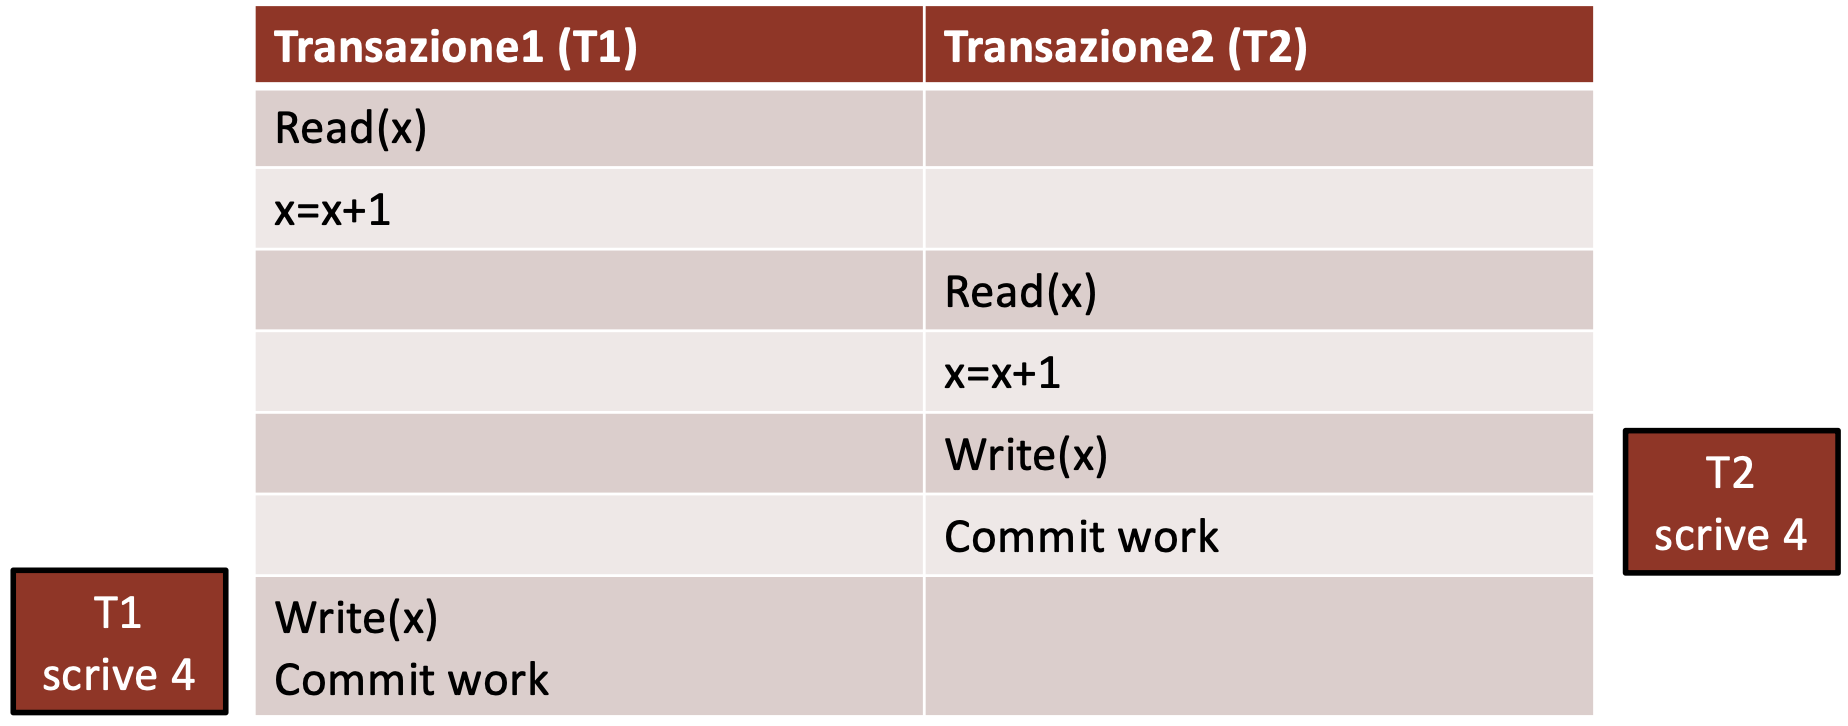
\includegraphics[width=0.8\textwidth]{foto 1.png}
    \end{center}
    In questo caso, l'esecuzione della seconda transazione invalida il risultato della prima transazione
    \item \textbf{Lettura sporca}
    \begin{center}
        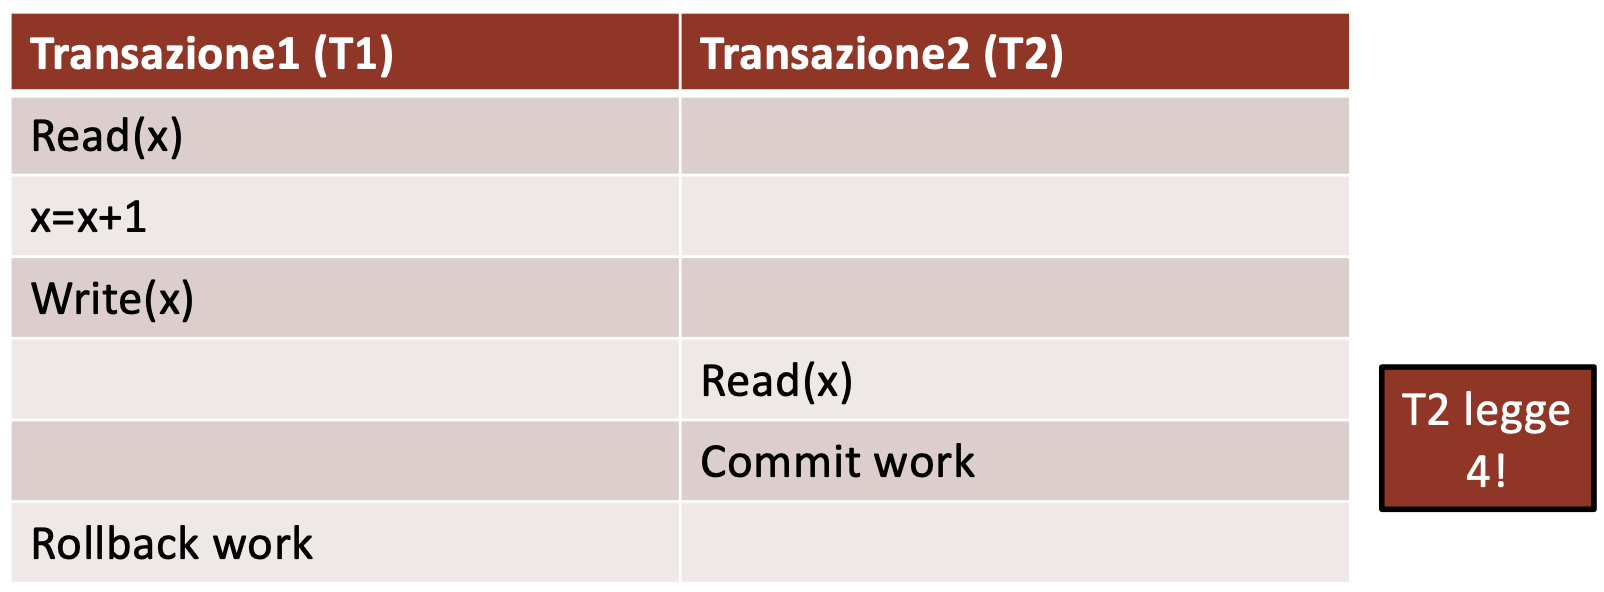
\includegraphics[width=0.8\textwidth]{foto 2.png}
    \end{center}
    Nel caso di rollback in una transazione, le transazioni che utilizzano quei dati compromessi si trovano in uno stato di errore
    \item \textbf{Letture inconsistenti}
    \begin{center}
        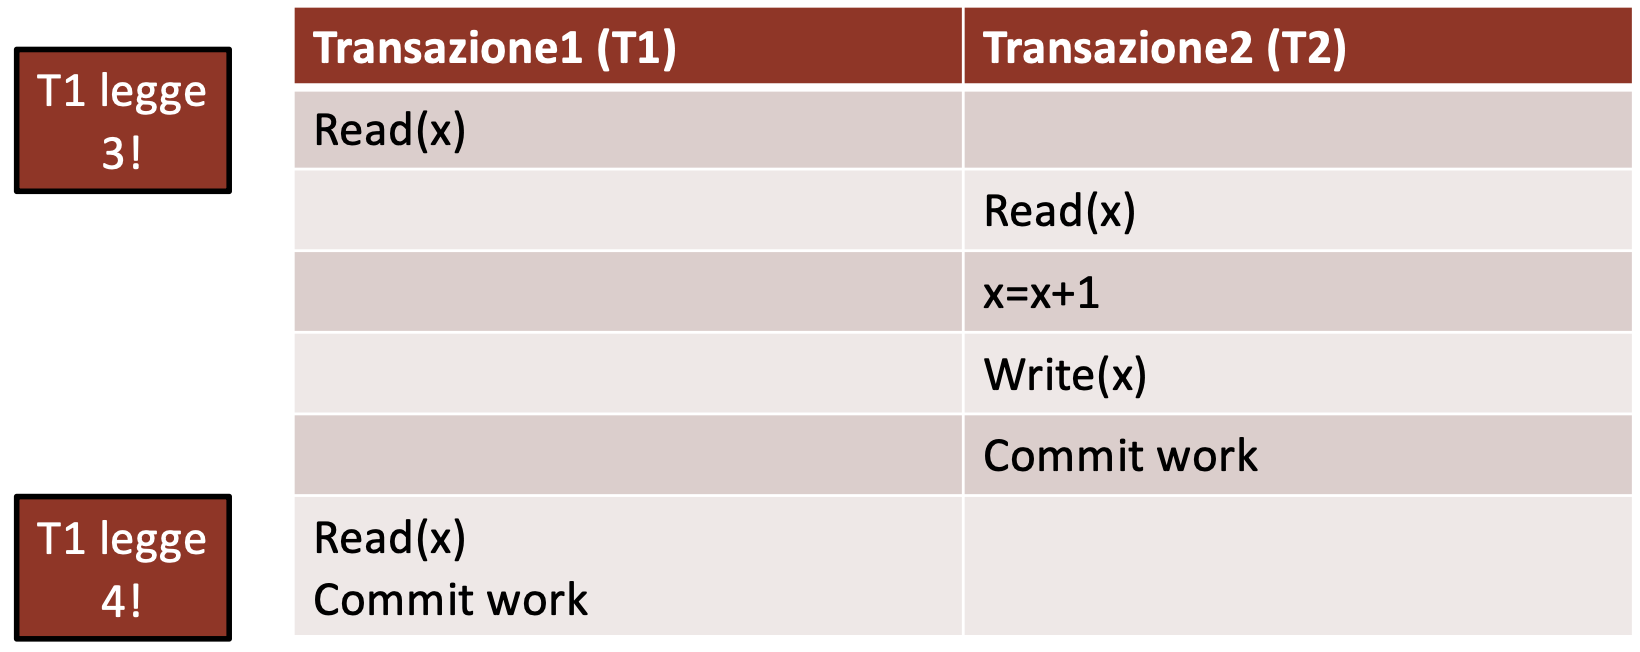
\includegraphics[width=0.8\textwidth]{foto 3.png}
    \end{center}
    In questo caso, viene effettuato un read precedente alla seconda transazione, che invalida il risultato richiesto
    \item \textbf{Aggiornamento fantasma}
    \begin{center}
        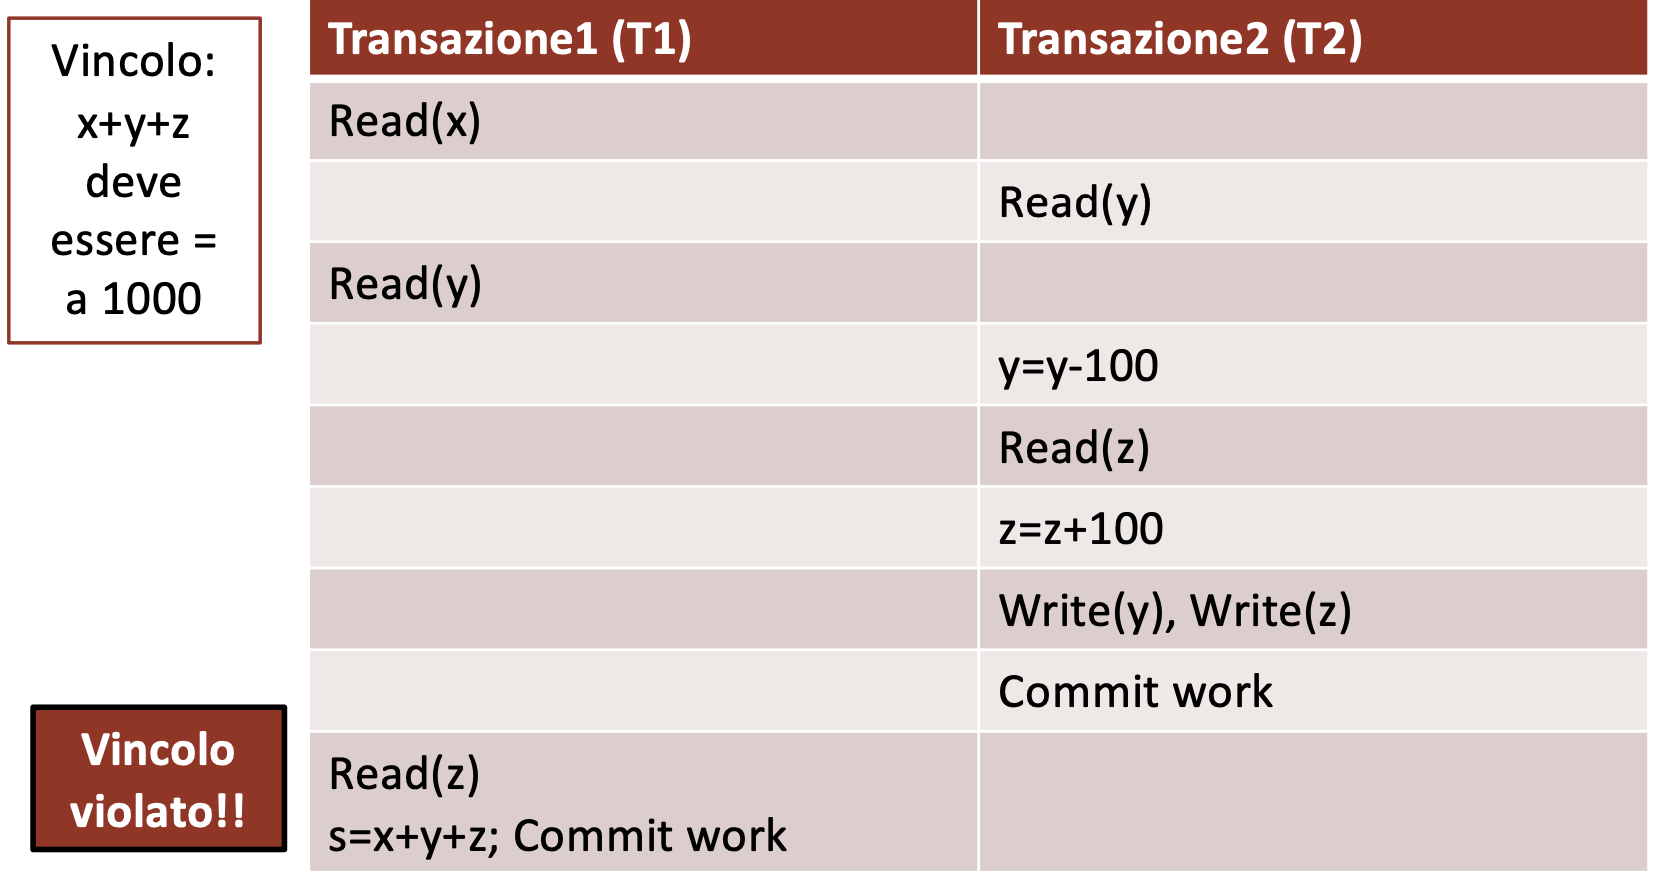
\includegraphics[width=0.8\textwidth]{foto 4.png}
    \end{center}
    In questo caso, la prima transazione non considera i valori modificati dalla seconda transazione, ottenendo un risultato errato
\end{enumerate}
Bisogna quindi stabilire un metodo per il \textbf{controllo della concorrenza}. I DBMS commerciali usano il meccanismo dei \textbf{lock}. Per poter effettuare una qualsiasi operazione di lettura/scrittura su una risorsa, tabella o valore di una cella, \textbf{è necessario aver precedenetemente acquisito il controllo, o lock, sulla risorsa stessa}. \\
Come visto in precedenza in altri corsi, il \textbf{lock in lettura} consente un accesso condiviso alla risorsa, mentre il \textbf{lock in scrittura} segue il concetto di mutua esclusione.\\
Su ogni lock possono essere definite \textbf{due operazioni}:
\begin{itemize}[label={-}, leftmargin=1cm]
    \item \textbf{Richiesta} del lock in lettura/scrittura
    \item \textbf{Rilascio} del lock acquisito in precedenza
\end{itemize}
\begin{center}
    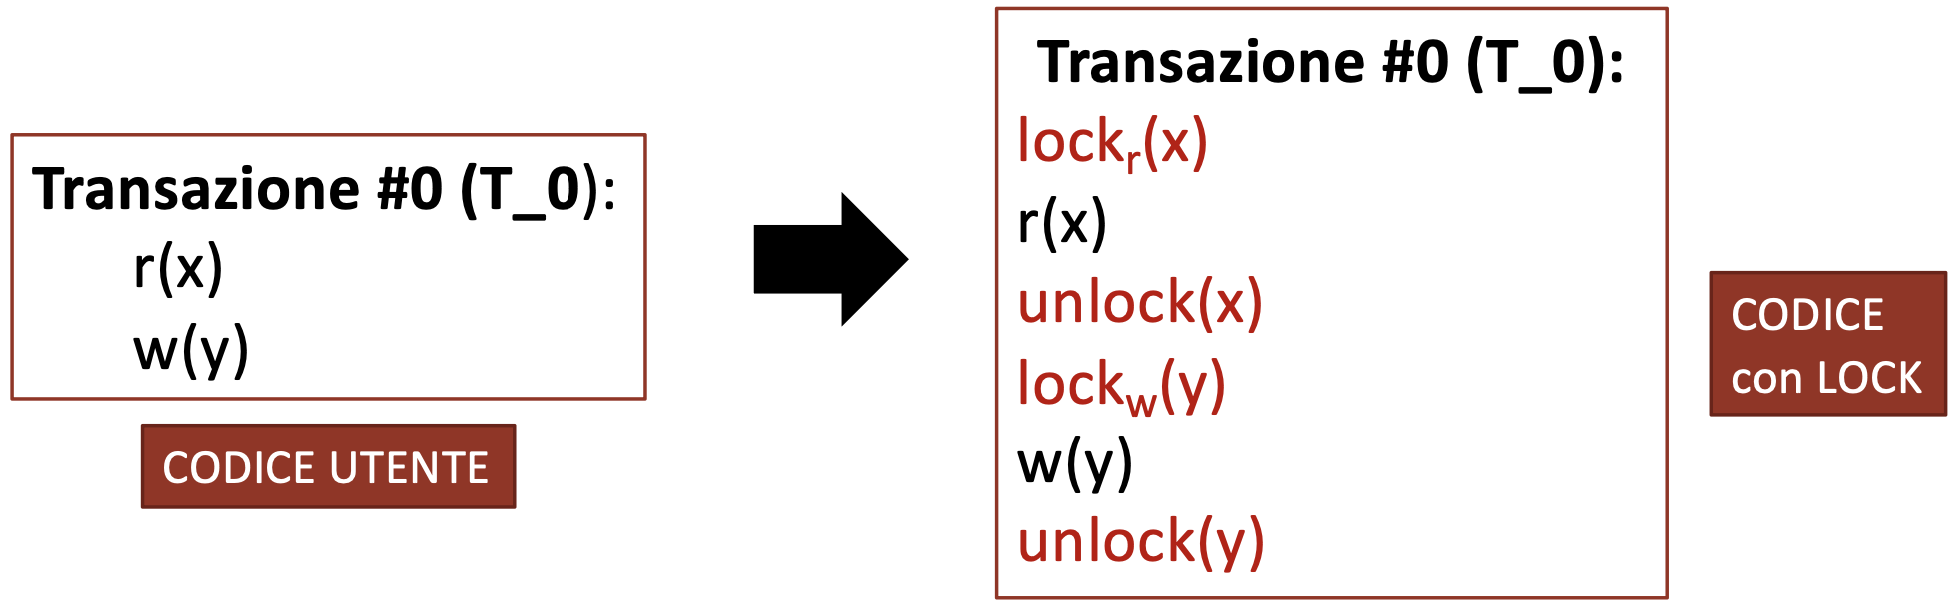
\includegraphics[width=0.65\textwidth]{foto 5.png}
\end{center}
Il \textbf{lock manager} è un componenete del DBMS responsabile di \textbf{gestire i lock alle risorse del DB, e di rispondere alle richieste delle transazioni}. Per ciascun oggetto \textit{x} del DBMS, possiamo accedere a tre strutture dati:
\begin{itemize}[label={-}, leftmargin=1cm]
    \item \textbf{State(x)}: indica lo \textbf{stato} dell'oggetto (libero / r\_locked / w\_locked)
    \item \textbf{Active(x)}: lista delle transazioni attive sull'oggetto
    \item \textbf{Queued(x)}: lista delle transazioni bloccate sull'oggetto
\end{itemize}
Davanti ad una richiesta, il lock manager esegue diversi step:
\begin{enumerate}[leftmargin=1cm]
    \item Riceve una richiesta (r\_lock / w\_lock / unlock) da una transazione \textit{T}, su un oggetto \textit{x}, che può essere una tabella, una colonna, etc
    \item Controlla la \textbf{tabella stato/azione}
    \begin{center}
        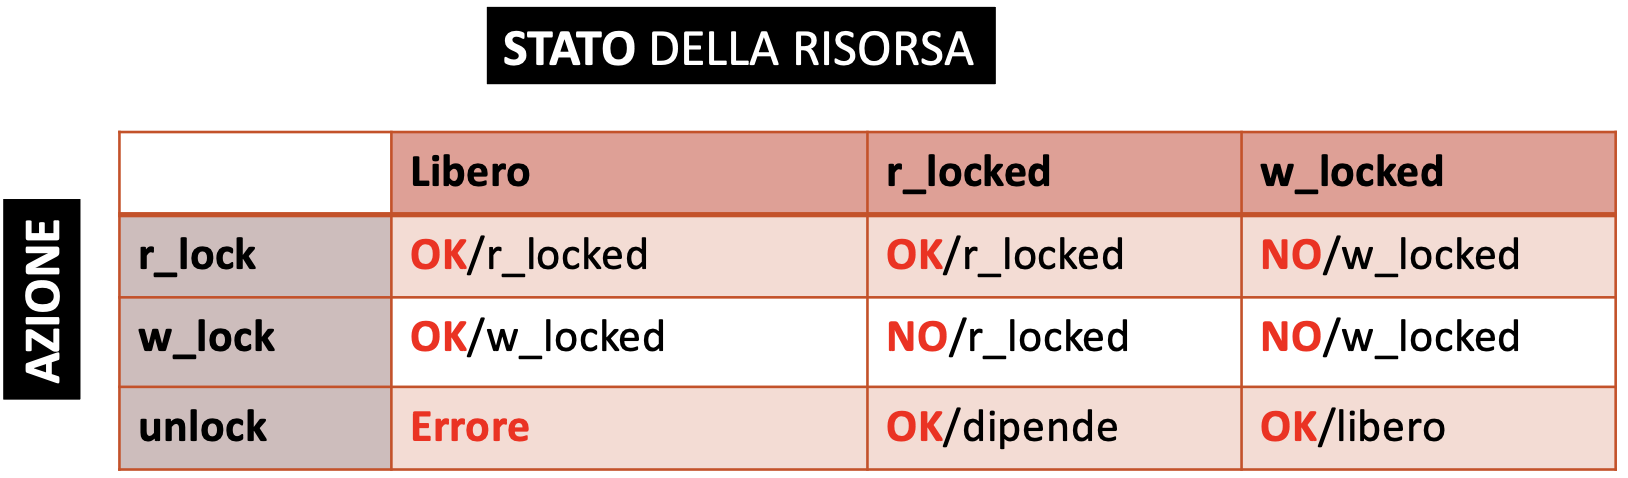
\includegraphics[width=0.65\textwidth]{foto 6.png}
    \end{center}
    \item Se la risposta è \textbf{OK}, \textbf{aggiorna lo stato della risorsa}, e concede il controllo della risorsa alla transazione \textit{T}
    \item Se la risposta è \textbf{NO}, \textbf{inserisce la transazione \textit{T} in una coda} associata ad \textit{x}
\end{enumerate}

\subsection*{Two Phase Lock (2PL)}
\large

In un \textbf{Two Phase Lock}, una transazione, \textbf{dopo aver rilasciato un lock, non può acquisirne un altro}. In pratica, una transazione \textbf{acquisisce prima tutti i lock delle risorse di cui necessita}.\\
Ogni schedule che rispetta il 2PL è anche \textbf{serializzabile}. Inoltre, ogni schedule che rispetta il 2PL non può incorrere in \textbf{configurazioni erronee} dovuta ad aggiornamenti fantasma, letture inconsistenti o perdite di aggiornamento; è ancora presente il problema della lettura sporca.

\subsection*{Strict Two Phase Lock (S2PL)}
\large

In un \textbf{Strict Two Phase Lock}, \textbf{i lock di una transazione sono rilasciati solo dopo aver effettuato le operazioni di commit/rollback}.\\
Uno schedule che rispetta lo S2PL \textbf{eredita tutte le proprietà del 2PL}, ed inoltre \textbf{non} presenta anomalie causate da problemi di \textbf{lettura sporca}.\vspace{14pt}\\
I due protocolli presentano un problema che li accomuna, potendo generare schedule con situazioni di \textbf{deadlock}. Per gestire le situazioni di deadlock causate dal lock manager, si possono usare tre tecniche:
\begin{enumerate}[leftmargin=1cm]
    \item \textbf{Uso dei timeout}: \textbf{ogni operazione di una transazione ha un timeout} entro il quale deve essere completata, \textbf{pena annullamento (rollback) della transazione stessa}
    \item \textbf{Deadlock avoidance}: prevenire le configurazioni che potrebbero portare ad un deadlock. Si può prevenire in due modi: attraverso l'utilizzo di \textbf{lock/unclock} di tutte le risorse allo stesso tempo; o attraverso l'utilizzo di \textbf{time stamp o di classi di priorità} tra transazioni (può provocare \textbf{starvation})
    \item \textbf{Deadlock detection}: utilizzare \textbf{algoritmi per identificare eventuali situazioni di deadlock}, e prevedere meccanismi di recovery dal deadlock. Si possono identificare attraverso l'utilizzo di \textbf{grafi delle richieste/risorse}, utilizzato per identificare la presenza di cicli. In caso di ciclo, si fa rollback delle transazioni coinvolte nel ciclo in modo da eliminare la mutua dipendenza\\
\end{enumerate}
MySQL offre quattro livelli di isolamento:
\begin{enumerate}[label={-}, leftmargin=1cm]
    \item \textbf{READ UNCOMMITTED}: sono visibili gli aggiornamenti non consolidati fatti da altri
    \item \textbf{READ COMMITTED}: aggiornamenti visibili solo se consolidati, ossia solo dopo COMMIT
    \item \textbf{REPEATABLE READ}: tutte le letture di un dato operate da una transazione leggono sempre lo stesso valore (comportamento di \textbf{default})
    \item \textbf{SERIALIZABLE}: lettura di un dato blocca gli aggiornamenti fino al termine della transazione stessa che ha letto il dato, lock applicato ad ogni SELECT\\
\end{enumerate}
Si osservi ora la sintassi generale in MySQL:\\
Per \textbf{iniziare una transazione} e completarla:
\begin{itemize}[label={ }, leftmargin=1cm]
    \item \textit{SET AUTOCOMMIT = 0}
    \item \textit{START TRANSACTION}
    \item \textit{\dots (Statements SQL)}
    \item \textit{COMMIT/ROLLBACK}
\end{itemize}
Per \textbf{configurare il livello di isolamento} di esecuzione:
\begin{itemize}[label={ }, leftmargin=1cm]
    \item \textit{SET TRANSACTION ISOLATION LEVEL}
    \item \quad \textit{REPEATABLE READ | READ COMMITTED | }
    \item \quad \textit{READ UNCOMMITTED | SERIALIZABLE}
\end{itemize}
\textit{Nota Bene}: le transazioni sono \textbf{utilizzabili solo} su tabelle di tipo \textbf{INNODB}.\vspace{14pt}\\
E' possibile inoltre \textbf{gestire manualmente le operazioni di lock} su tabelle, anche se sconsigliato su tabelle di tipo INNODB:
\begin{itemize}[label={ }, leftmargin=1cm]
    \item \textit{LOCK TABLES}
    \item \quad \textit{tabella {READ | WRITE}}
\end{itemize}
\end{document}